\section{Runs Submitted to Clef Selection}
\label{sec:runs_selection}

\begin{table}[h!]
    \begin{center}
        \caption{MAP and NCDG scores for all runs in training data}
        \label{tab:all_scores}
        \begin{tabular}{|c|c||c|c|}
            \hline
            \textbf{Run ID} & \textbf{Run} & \textbf{MAP Score} & \textbf{NCDG Score}\\
            \hline\hline
            01 & en\_en & \cellcolor{red!30!white}0.0700 & \cellcolor{red!30!white}0.1614 \\
            \hline
            02 & en\_en\_3gram & 0.0704 & 0.1661 \\
            \hline
            03 & en\_en\_4gram & 0.0874 & 0.2025 \\
            \hline
            04 & en\_en\_5gram & 0.1028 & 0.2288 \\
            \hline
            05 & en\_en\_fr\_5gram & \cellcolor{red!60!white}0.0669 & \cellcolor{red!60!white}0.1525 \\
            \hline
            06 & en\_en\_4gram\_ner & \cellcolor{red}0.0360 & \cellcolor{red}0.1098 \\
            \hline
            07 & fr\_fr & 0.1656 & 0.3135 \\
            \hline
            08 & fr\_fr\_3gram & \cellcolor{green!30!white}0.1698 & \cellcolor{green!30!white}0.3208 \\
            \hline
            09 & fr\_fr\_4gram & \cellcolor{green!60!white}0.1737 & \cellcolor{green!60!white}0.3269 \\
            \hline
            10 & fr\_fr\_5gram & \cellcolor{green}0.1748 & \cellcolor{green}0.3285 \\
            \hline
            11 & fr\_en\_fr\_5gram & 0.1288 & 0.2797 \\
            \hline
            12 & fr\_fr\_4gram\_ner & 0.1362 & 0.2881 \\
            \hline
        \end{tabular}
    \end{center}
\end{table}

% Ferro said that with this data we should only use the tables
%\begin{figure}[h!]
%    \centering
%    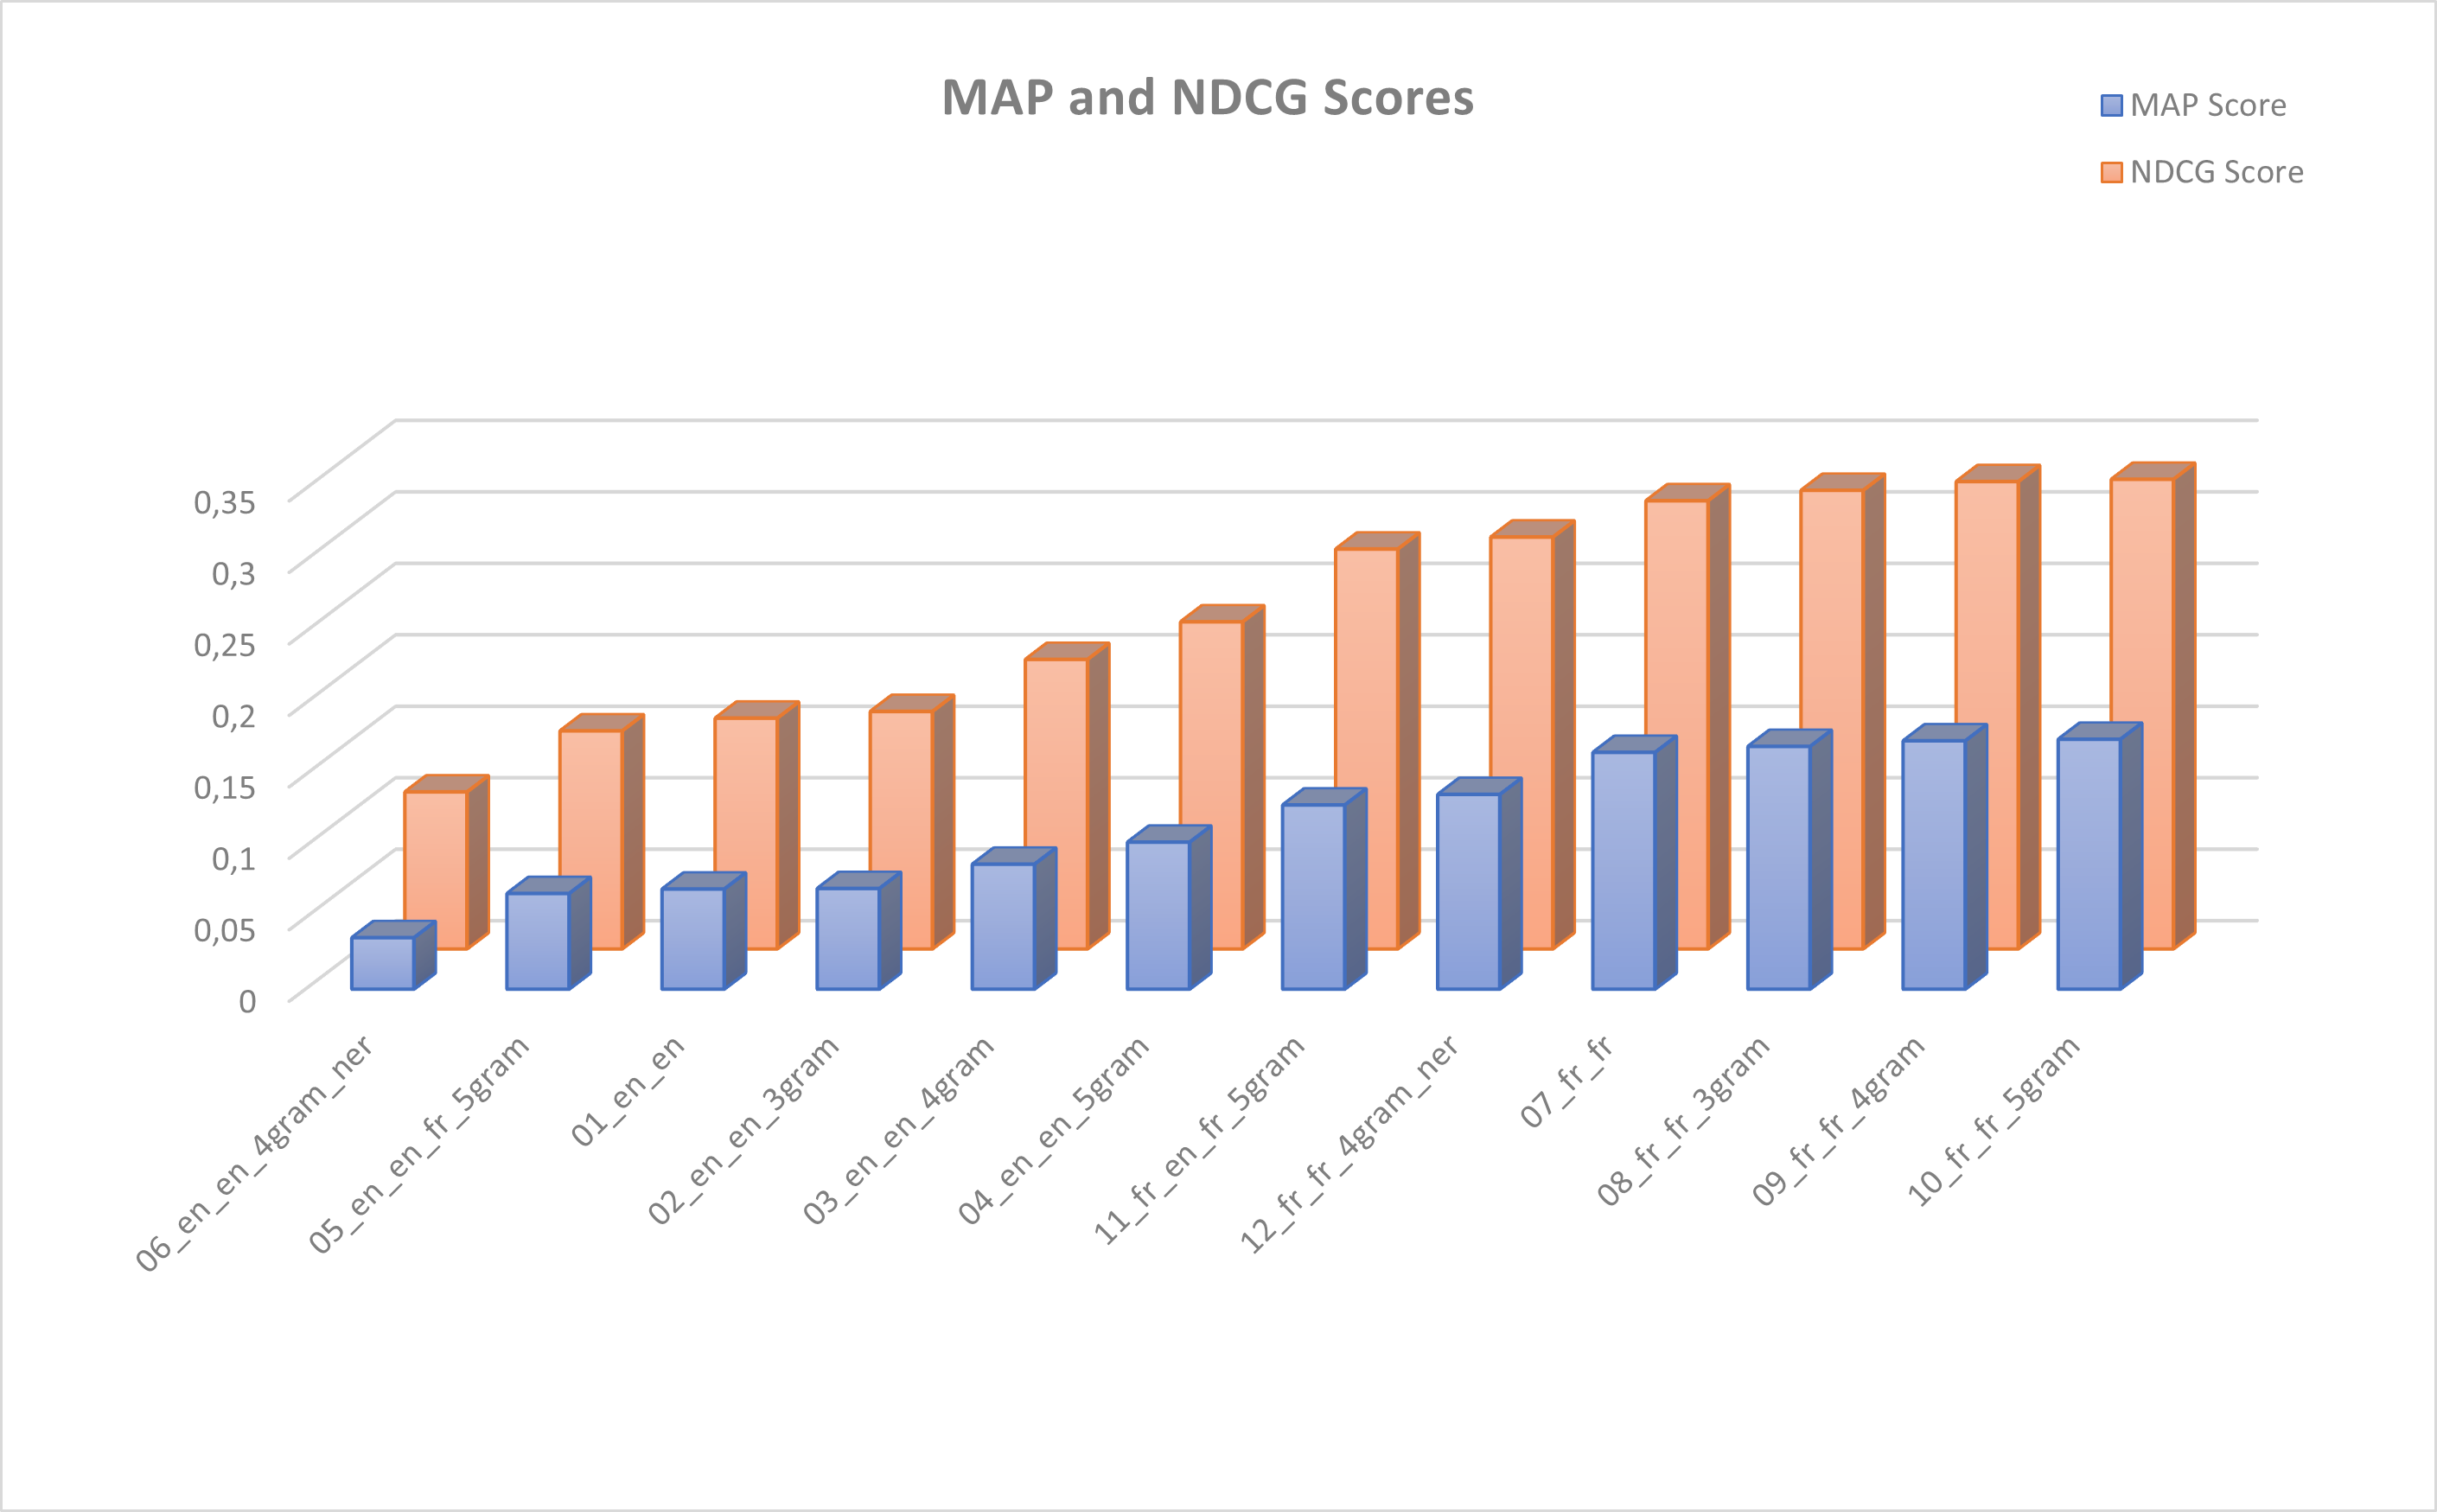
\includegraphics[width=0.6\textwidth]{figure/allScores}
%    \caption{All scores sorted by MAP score}
%    \label{fig:sorted_scores}
%\end{figure}

The analysis shows that the highest MAP score (0.1748) is achieved by \texttt{10\_fr\_fr\_5gram}, followed by
\texttt{09\_fr\_fr\_4gram} (0.1737),
\texttt{08\_fr\_fr\_3gram} (0.1698),
\texttt{07\_fr\_fr} (0.1656), and
\texttt{12\_fr\_fr\_4gram\_ner} (0.1362).
The lowest MAP score (0.0360) is obtained by \texttt{en\_en\_4gram\_ner}.

Similarly, the highest NDCG score (0.3285) belongs to \texttt{10\_fr\_fr\_5gram}, followed by
\texttt{09\_fr\_fr\_4gram} (0.3269),
\texttt{08\_fr\_fr\_3gram} (0.3208),
\texttt{07\_fr\_fr} (0.3135), and
\texttt{12\_fr\_fr\_4gram\_ner} (0.2881).
The lowest NDCG score (0.1098) corresponds to \texttt{en\_en\_4gram\_ner}.\\

Because of this, the five system submitted to CLEF have been (in order of importance): \texttt{10\_fr\_fr\_5gram},
\texttt{09\_fr\_fr\_4gram}, \texttt{08\_fr\_fr\_3gram}, \texttt{07\_fr\_fr}, \texttt{12\_fr\_fr\_4gram\_ner}.
Following the competition workflow, we created new indexes based on the test data and re-executed this top five runs.\\

% Ferro said that with this data we should only use the tables
%Here we can see a chart ranking of the five best scores, they are the runs that have been presented at CLEF:
%\begin{figure}[h!]
%    \centering
%    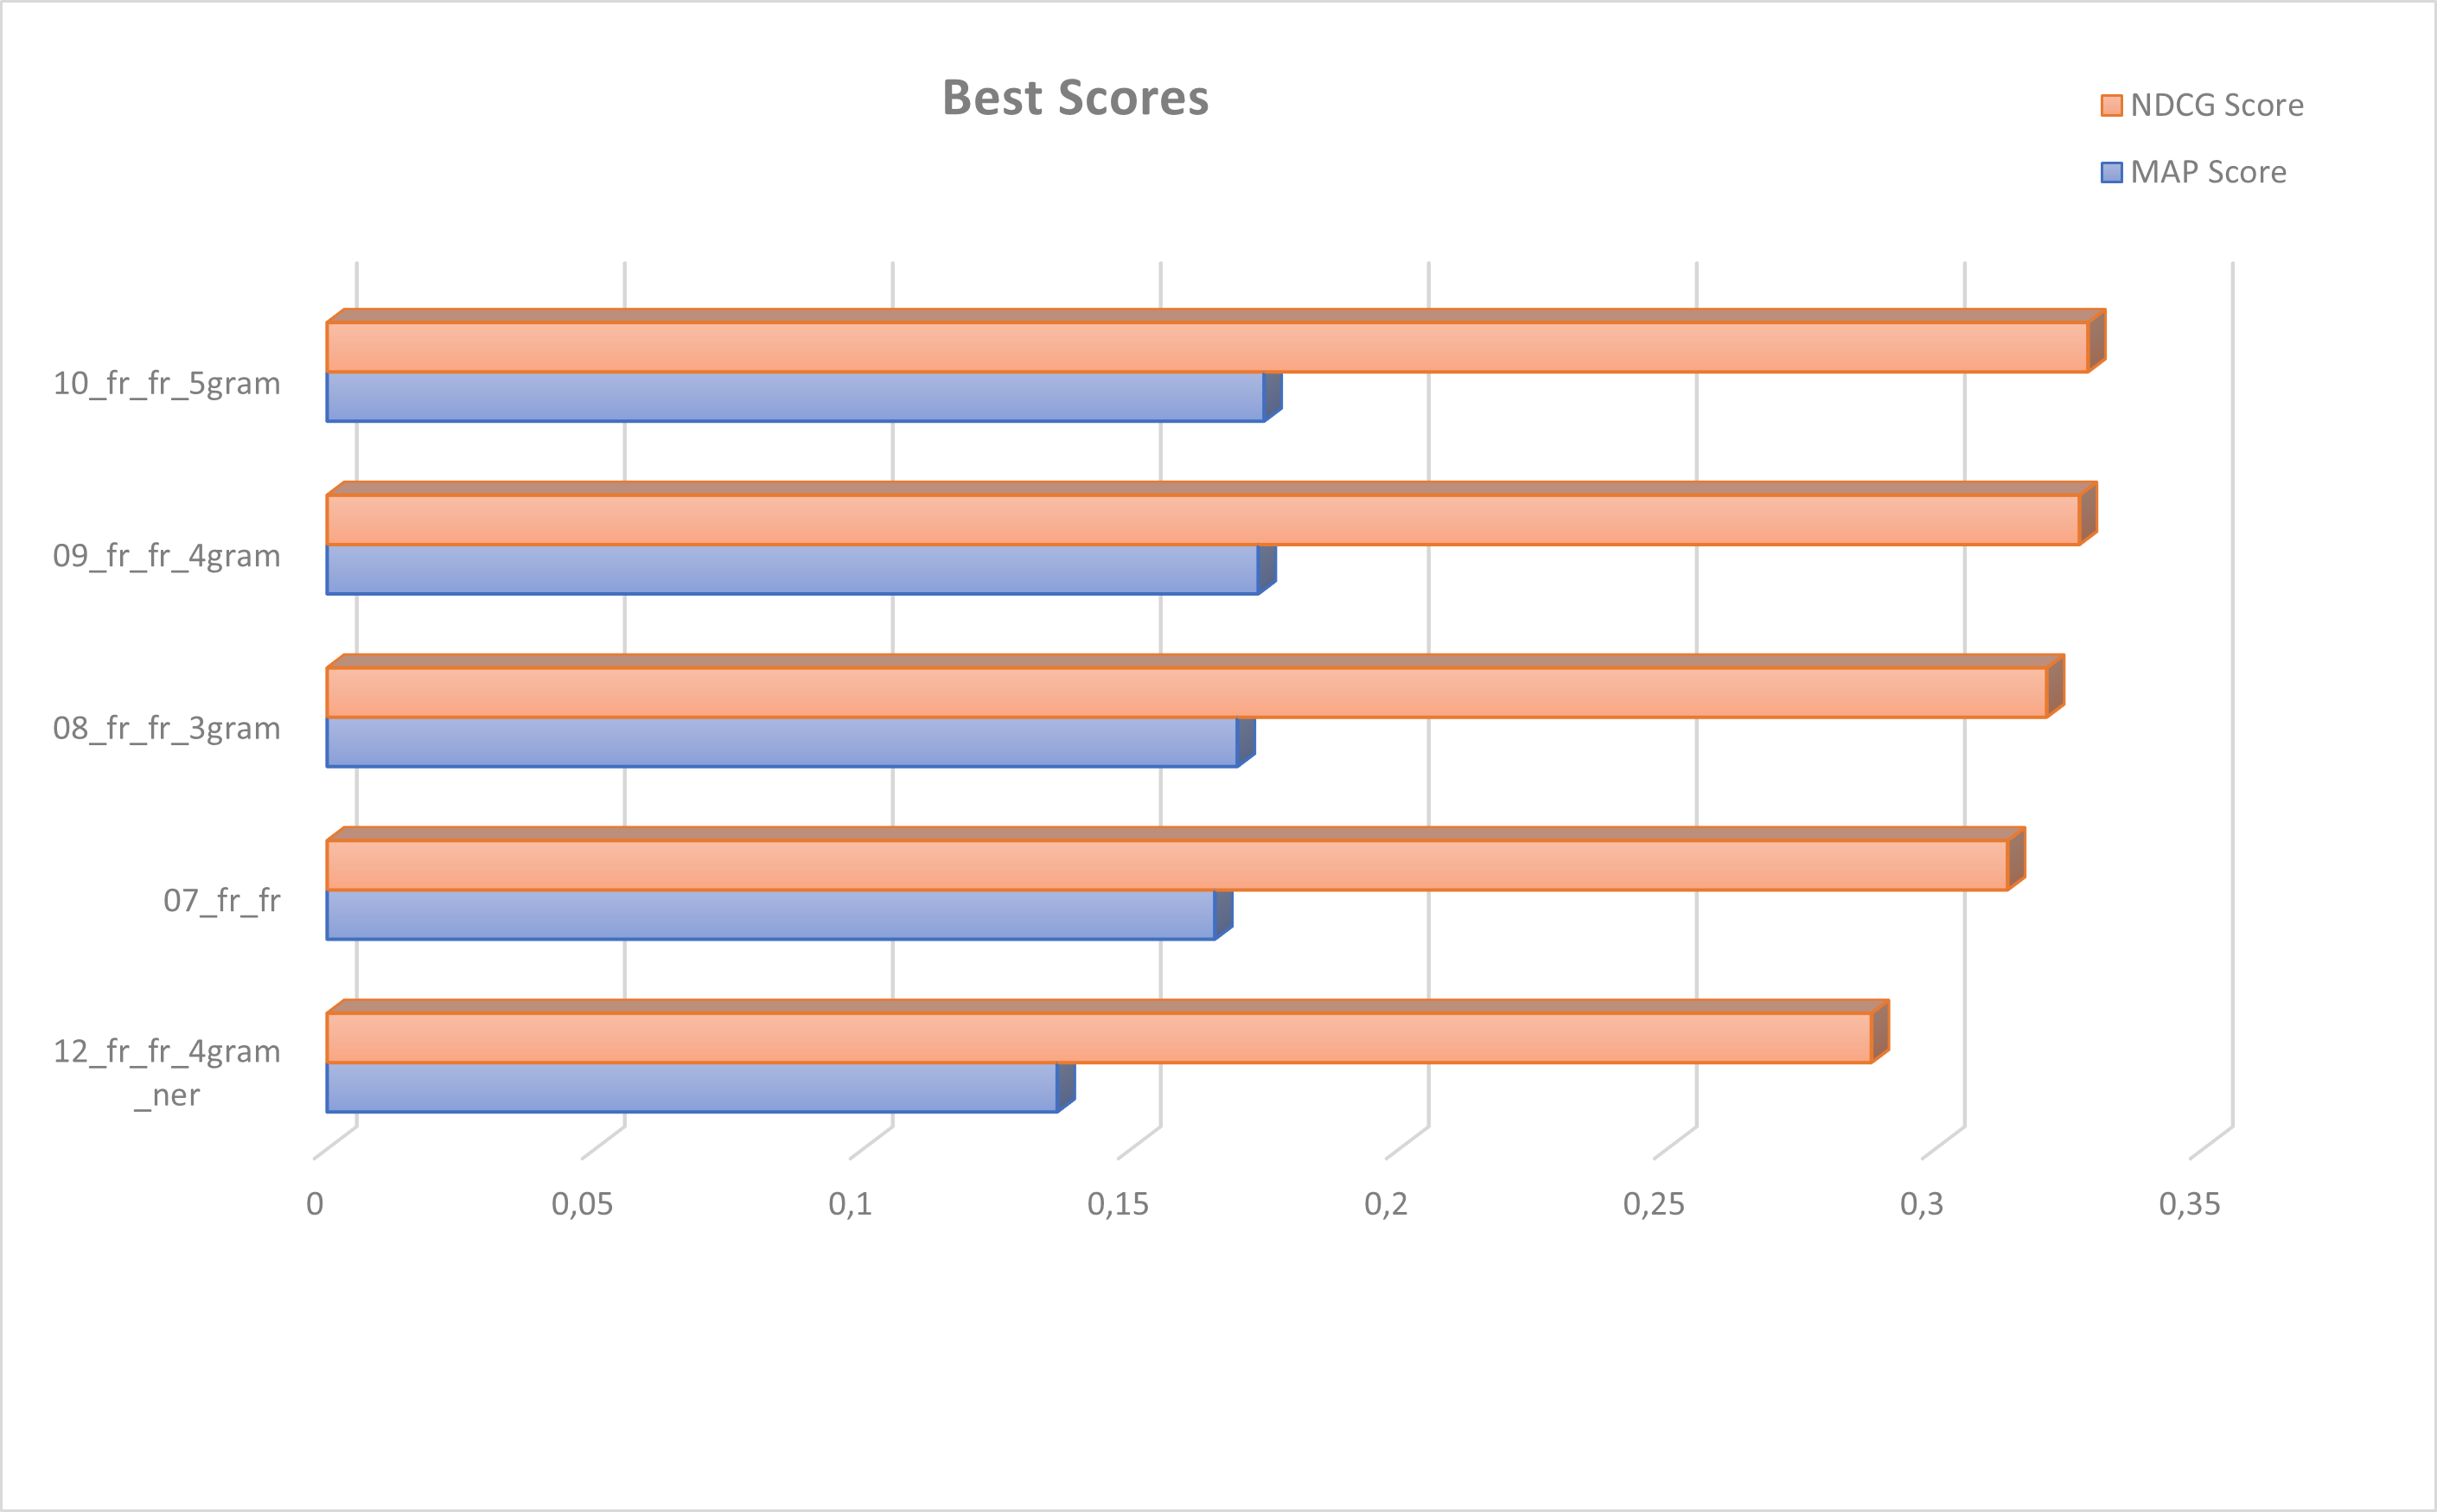
\includegraphics[width=0.6\textwidth]{figure/bestScores}
%    \caption{Best MAP and NDCG scores}
%    \label{fig:best_scores}
%\end{figure}